\documentclass[11pt]{article}
\usepackage[T1]{fontenc}
\usepackage[utf8]{inputenc}
\usepackage[sort]{natbib}
\usepackage{amsmath, amssymb}
\usepackage{fancyhdr}
\usepackage{dsfont}
\usepackage{graphicx}
\usepackage{float}
\usepackage{subfig}
\usepackage{pdfpages}

%\usepackage{fancyvrb}

%‎\usepackage{caption}‎
%‎\usepackage{color,xecolor}‎
%‎\usepackage[framed,numbered,autolinebreaks,useliterate]{mcode}‎
%\lstset{breakatwhitespace=false}
\usepackage[numbered, autolinebreaks, framed]{mcode}		% codice matlab
%\lstset{breaklines=true,breakatwhitespace=true,prebreak=\usebox{\lbreakdots}}
\usepackage{enumitem}						% elenco puntato
\renewcommand{\labelenumi}{\alph{enumi}.} 	% Make numbering in the enumerate environment by letter rather than number (e.g. section 6)	


%----- you must not change this -----------------
\oddsidemargin 0.2cm
\topmargin -1.0cm
\textheight 24.0cm
\textwidth 15.25cm
\parindent=0pt
\parskip 1ex
\renewcommand{\baselinestretch}{1.1}
\pagestyle{fancy}
\setlength{\headheight}{14pt}

%----------------------------------------------------



% enter your details here----------------------------------

\lhead{\normalsize \textrm{Roberto Costa}}
\chead{\normalsize Matricola: 1128285}
\rhead{Lab. 3}
\lfoot{\normalsize \textrm{Image and Video Anlysis}}
\cfoot{\thepage}
\rfoot{\normalsize Matricola: 1128285}
\setlength{\fboxrule}{4pt}\setlength{\fboxsep}{2ex}
\renewcommand{\headrulewidth}{0.4pt}
\renewcommand{\footrulewidth}{0.4pt}

\title{LABORATORY \#5: REPORT \\ A.A. 2015-2016} 
\author{Roberto \textsc{Costa}} % Author name
\date{\today}

\begin{document}
\maketitle
\begin{center}
\begin{tabular}{l r}
Subject: & Image and Video Analysis\\
Delivery date: & 19-05-2016 \\ 
Professor: & P. Zanuttigh \\
Student number: & 1128285
\end{tabular}
\end{center}


% If you wish to include an abstract, uncomment the lines below
%\begin{abstract}
% Abstract text
%\end{abstract}

\section{Algorithm developed}
\begin{lstlisting}
close all;
clear all;
addpath('lib');
global method
global MAX_FRAMES
global T1
global alpha
global T3
global R
global sigma
global T4
MAX_FRAMES  = 50;
T1 = 1/255;
alpha = 0.7;
T3 = 7/255;
R = 5;
sigma = 0.2;
T4 = 0.4;

%[movRGB, f_rate] = read_video('../video/lab2016_1.mp4');
%save('movRGB.mat','movRGB', 'f_rate');
load('movRGB.mat');
methods = {'Fixed Threshold','Background modeling','Probabilistic Approach'};
instant = 25;
for i=1:3
    method = i;
    disp(strcat('Method: ',methods(method)));
    motion = motion_detection(movRGB);
    %implay(mov/255, f_rate);
    results(:,:,method) = motion(:,:,instant);
end
implay(motion, f_rate);

for i=1:3
    figure(i);
    imshow(results(:,:,i));
end
figure(4);
imshow(movRGB(:,:,:,instant)/255);
\end{lstlisting}

Where the function 'motion\_detection' has the following code:
\begin{lstlisting}
function motion = motion_detection(movRGB)
%% SOME USEFUL GLOBAL VARIABLES
global method
global T1
global alpha
global T3
global R
global sigma
global T4

%% CONVERTING RGB IMAGE TO GREYSCALE IMAGE
[h, w, ~, t] = size(movRGB);
motion = zeros(h,w,t-1);
mov = zeros(h,w,t);
for k=1:t
    mov(:,:,k)=rgb2gray(movRGB(:,:,:,k)/255);
end

%% FIXED THRESHOLD METHOD
if (method==1)
    for k=2:t
        rho = mov(:,:,k)-mov(:,:,k-1);
        motion(:,:,k-1) = rho.^2 > T1;
    end
end

%% BACKGROUND MODELING METHOD
if (method==2)
    B = zeros(h,w,t-1);
    B(:,:,1) = mov(:,:,1);
    for k=2:t
        B(:,:,k) = alpha * mov(:,:,k-1) + (1-alpha)*B(:,:,k-1);
        rho = mov(:,:,k)-B(:,:,k);
        motion(:,:,k-1) = rho.^2>T3;
    end
end

%% PROBABILISTIC APPROACH
if (method==3)
    Pbgr = zeros(h,w,t-1);
    for k = 2:R
        for i=1:k-1
            Pbgr(:,:,k-1) = Pbgr(:,:,k-1) + ...
                exp(-1/(2*sigma^2)*(mov(:,:,k)-mov(:,:,k-i)).^2)/(k-1);
        end
        motion(:,:,k-1) = Pbgr(:,:,k-1) <= T4;
    end
    for k = R+1:t
        for i=1:R
            Pbgr(:,:,k-1) = Pbgr(:,:,k-1) + ...
                exp(-1/(2*sigma^2)*(mov(:,:,k)-mov(:,:,k-i)).^2)/R;
        end
        motion(:,:,k-1) = Pbgr(:,:,k-1) <= T4;
    end
end
\end{lstlisting}
\section{Results}
\begin{figure}[H]
	\centering
	{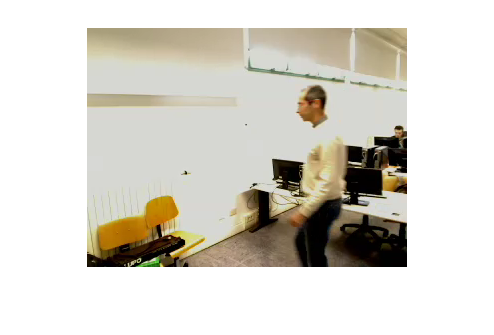
\includegraphics[width=12cm]{images/inst.png} }
    \caption{Input video at a certain instant}
    \label{fig:out1}
\end{figure}
\begin{figure}[H]
	\centering
	{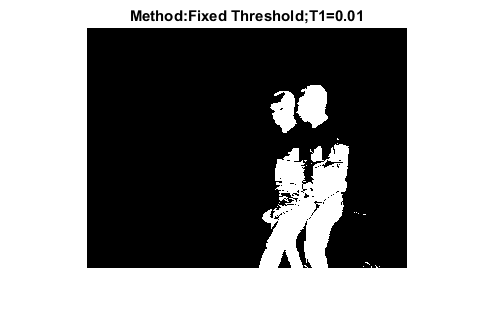
\includegraphics[width=12cm]{images/inst_1.png} }
    \caption{Output video at a certain instant with method 1}
    \label{fig:out1}
\end{figure}
\begin{figure}[H]
	\centering
	{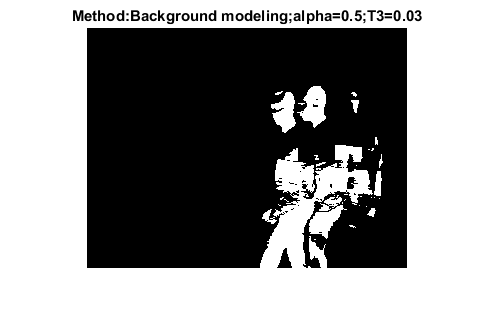
\includegraphics[width=12cm]{images/inst_2.png} }
    \caption{Output video at a certain instant with method 2}
    \label{fig:out2}
\end{figure}
\begin{figure}[H]
	\centering
	{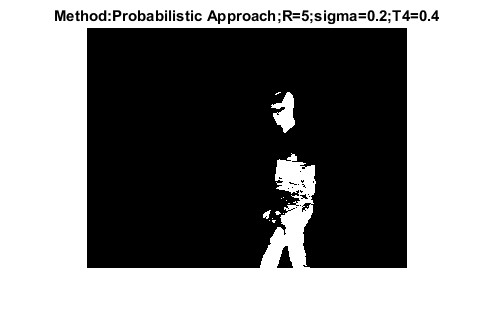
\includegraphics[width=12cm]{images/inst_3.png} }
    \caption{Output video at a certain instant with method 3}
    \label{fig:out3}
\end{figure}


\end{document}
